\documentclass[main.tex]{subfiles}

\pagestyle{fancy}
\fancyhf{}
\fancyhead[LE]{\makebox[\pageoffset][l]{\bfseries\thepage}\bfseries\leftmark}
\fancyhead[RO]{\bfseries\rightmark\makebox[\pageoffset][r]{\bfseries\thepage}}

\begin{document}
\label{chap:Force}

\section*{Goal}
This week, we will look into how the dynamics of motion of an object can change with different amounts of net force. We will also examine the relationship between the applied force, acceleration, and the mass of an object.

\section*{Equipment}
\begin{itemize}
\item
850 Universal Interface (850UI)
\item
PASCO Capstone
\item
Dynamics track and cart
\item
Masses and string
\item
Photogate with Pulley, Motion Sensor, Force Sensor
\item
Triple-Beam Balance
\end{itemize}•

\section*{Theory}
Isaac Newton described the relationship of the net force applied to an object and the acceleration it experiences in the following way: the acceleration ($a$) of an object is directly proportional to and in the same direction as the net force ($F_{net}$), and inversely proportional to the mass ($m$) of the object:
\begin{equation} \label{eq:Law2}
a=\frac{F_{net}}{m}
\end{equation}
Consider the system illustrated below. A cart of mass $M$ on a horizontal track is attached via a ``frictionless, massless" pulley to a vertically hanging mass $m.$ We can show that for this specific situation, that the acceleration of the cart rolling along the track will be,
\begin{equation} \label{eq:acc_cart}
a=\frac{mg}{M+m}.
\end{equation}•
(This can be found using free body diagrams, and will be discussed in lab.) Using Newton's Second Law, we can then say that the tension on the string, and thus the net force on the cart is,
\begin{equation} \label{eq:F_cart}
T=Ma=\frac{Mmg}{M+m}
\end{equation}

\section{Setup I: Acceleration and Force of a Cart.}
\begin{enumerate}
\item
Open Capstone
\item
Attach the Photogate to the 850UI and tell Capstone what port the sensor is plugged into. Make sure to select the \emph{``Photogate with Pulley"} in Capstone. This will automatically load the proper settings for the Photogate when we are using it with a pulley.
\item
Hide the ``Hardware Setup" and double-click on ``Graph" in the toolbar to the right.
\item
For the vertical axis choose ``Linear Speed (m/s)."
\item
Arrange the dynamics track, cart and pulley as shown. Level the track so that the cart will not roll one way or the other on its own.

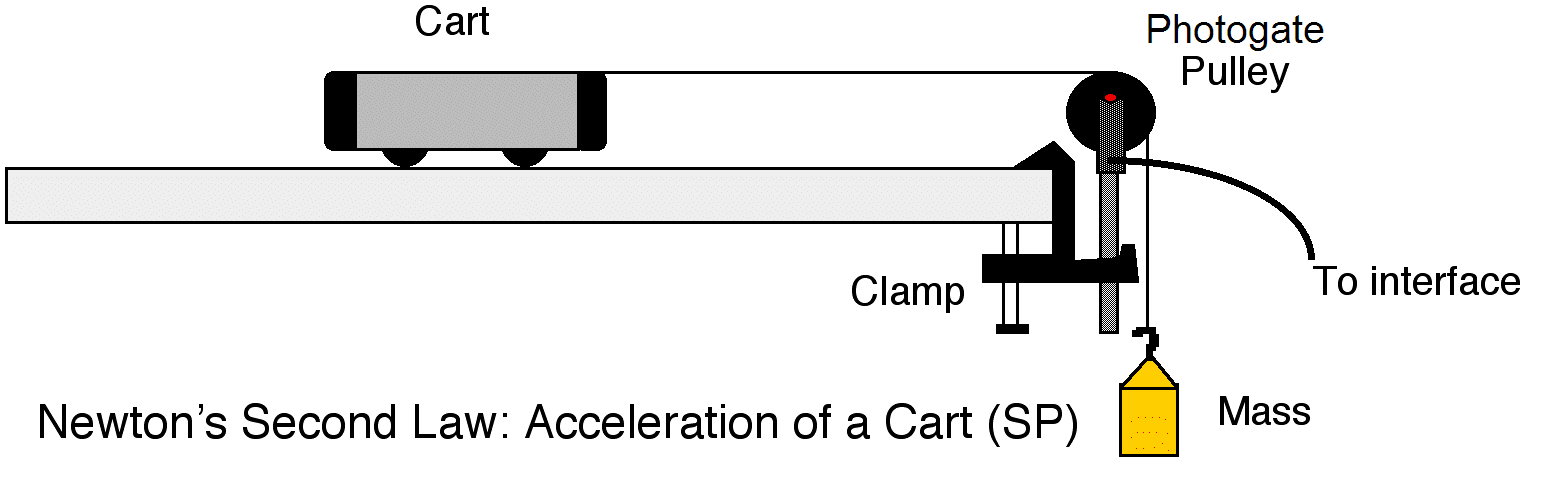
\includegraphics[width=\textwidth]{Force_1_Setup}

\item
Attach a string to the dynamics cart. Make the string long enough so that when the cart is next to the Pulley and the string is over the pulley, the string reaches the ground. Attach a mass hanger to the other end of the string. Put the string that connects the cart and the mass hanger over the Pulley. Adjust the Pulley so that the string from the cart is parallel to the level track or the top of the table.
\item
Place about 20 grams of mass on the 50 gram mass hanger so that the total initial hanging mass is 70 grams. Add about 200 grams of mass to the top of the cart.
\end{enumerate}•

\subsection*{Procedure}
\begin{enumerate}
\item
Measure and record the total mass of the cart ($M$) in the data table provided.
\item
Measure and record the total mass of the mass hanger and masses ($m$).
\item \label{step:Force1_start}
When we are ready to collect data, pull the cart away from the Photogate Pulley until the mass hanger almost touches the pulley. Turn the pulley so that the photogate beam of the Smart Pulley is “unblocked” (the light-emitting diode (LED) on the photogate is off).
\item
Click the Record button to begin data recording. Release the cart so it can be pulled by the falling mass hanger. Data recording will begin when the Pulley photogate is first blocked. 
\item
Stop the data recording just before the mass hanger reaches the floor by clicking ``Stop."  n.b., Do not let the cart hit the Pulley as it could damage it.
\item \label{step:Force1_end}
In the graph window, rescale the data by using the Scale to Fit button 
\includegraphics{Rescale}. Fit a linear line to the data. The slope of the line is the acceleration of the cart. Record this value in the data table provided.
\begin{question}
Why is the the slope of this line the acceleration of the cart?
\end{question}
\item
Change the applied force by moving masses from the cart to the hanger. This changes the force without changing the total mass. Measure and record the new values for $M$ (total mass of cart) and $m$ (mass hanger and masses).
\item
Repeat steps~\ref{step:Force1_start}--\ref{step:Force1_end} for a total of at least five times. Each time, move some mass from the cart to the mass hanger. Measure and record the values for $M$ (cart) and $m$ (mass hanger and masses). Record the value of the slope for each trial. \textbf{Print} the graph of the last trial for each group member.
\end{enumerate}•

\subsection*{Analysis}
\begin{enumerate}
\item \label{step:Analysis_Tacc}
Calculate the theoretical acceleration using Equation~\eqref{eq:acc_cart}. Record the theoretical acceleration in the data table.
\item
Calculate the net force acting on the cart for each trial. The net force on the cart is the tension in the string minus the friction forces. If friction is neglected, the net force is,
\[
F_{net}=M_{cart}a,
\]
where $a$ is the theoretical acceleration from step~\ref{step:Analysis_Tacc}.
\item
Find an experimental net force on the cart using $M$ (mass of cart) and the experimental acceleration.
\item
Calculate the percent discrepancy between the experimental and theoretical forces. 
\item
Also calculate the total mass $(M+m)$ that is accelerated in each trial.
\end{enumerate}•

\begin{question}
What is the relationship between force and acceleration?
\end{question}

\section{Setup II: Measuring Force on a cart directly.}
Here we will be using the same experimental setup as before but with one addition. We will now mount a force sensor to the top of the cart and attach the string to the sensor. The force sensor is a device that we can use to measure how much force is being applied on the hook. The hook is connected to a variable resistor so that when the hook is pulled or pushed the circuit reads the change in voltage and sends that information to Capstone. Capstone then assigns certain voltage values to specific force values. While Capstone does use a default setting, we will often calibrate the force sensor manually ourselves.
\begin{enumerate}
\item
Use the same setup as in part one. Delete any data from that part. The Graph window should be displaying ``Linear Speed versus Time." 
\item
Attach a Force Sensor to the Analogue channel ``A" on the 850UI.
\item
In Capstone, under ``Hardware Setup" click on the port that the force sensor is plugged into and add the sensor. There are a few versions of the Force Sensor in Capstone, the one that we will always use is simply called ``Force Sensor."
\item
Create a table for the Force data by double-clicking the ``Table" button in the toolbar on the right. This will create a table in the same window as our graph. For the first column choose ``Force (N)" to be the measurement, ``Time (s)" for the second column.
\item
We need to calibrate the Force Sensor.
\begin{enumerate} \label{page:Calibration}
\item
Mount the Force Sensor on a horizontal rod so that the sensor's hook is pointing downwards. Do \emph{not} put an object on the hook yet.
\item
In the toolbar on the left, there is a button labeled ``Calibration." Click on this. We will follow the on-screen instructions. We will be calibrating Force.
\item
In step 3, we will be using the ``Two Standards (2 point)" option.
\item
For the first point we will set our ``zero point." Press the tare button on the side of the physical force sensor. In Capstone set the standard value to be 0 N and press the ``Set Current Value to Standard Value" button, then click ``Next."
\item
For the second point, hang an object of known mass, e.g., 1 kg or 0.5 kg works best.
\item
Type in the object's weight in Newtons for the Standard Value. For this experiment, we will want to enter this value as negative to indicate that the force is pulling away from the sensor. Press the ``Set Current Value to Standard Value" button, then click ``Next."
\item
We should be presented with a summary of the calibration. Press ``Finish" to complete the calibration then click the ``Calibration" button on the left to hide the window.
\end{enumerate}•
\item
Carefully measure and record the mass of the cart and the Force Sensor $M.$ The cart and sensor are too massive for the balance to measure together so we will need to measure them separately.
\item
Use a \# 0 Phillips head screwdriver to mount the Force Sensor onto the accessory tray of the cart. 
\item
Use a string that is 10 cm longer than the length needed to reach the floor when the cart is next to the pulley. Attach one end to the Force Sensor's hook.

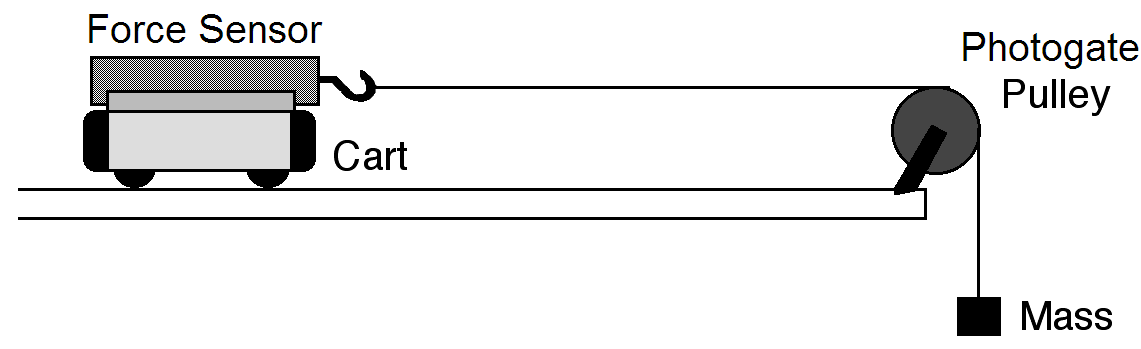
\includegraphics[width=\textwidth]{Force_2_Setup}

\item
Add 20 or 30 grams to the mass hanger. Carefully measure and record the total mass $m.$
\item
Attach the mass hanger to the other end of the string and put the string in the pulley's groove. Adjust the height of the pulley so that the string is parallel to the track.
\end{enumerate}•

\subsection*{Procedure}
\begin{enumerate}
\item
Pull the cart toward the left end of the track, and don't let the mass hanger bump into the pulley.
\item
Click the Record button to begin data collection and then release the cart.
\item
Click Stop to end recording just before the cart reaches the pulley. Stop the cart before it collides with the pulley.
\item
In the \emph{Graph} rescale the data by clicking the Scale To Fit button. Fit a linear line to the data. The slope of the straight line is the acceleration. 
\item
In the \emph{Table} click on the small triangle to the right of the Show Selected Statistics button 
\includegraphics{Statistics}. Check the Mean and Standard Deviation choice and uncheck everything else. Click on the $\Sigma$ to actually show the results.
\item
\textbf{Print} a copy of the Graph and Table for all group members.
\end{enumerate}•

\subsection*{Analysis}
\begin{enumerate}
\item
In the Graph of the velocity of the cart, use the Selection tool 
\includegraphics{Selection_Tool} to create a rectangle around the region of the plot that shows the movement of the cart. Record the value of the acceleration $a_{exp}$ (slope) for this region in the data table provided.
\item
Note the beginning and ending times of your selected rectangle.
\item
In the Table of the force on the cart, click on the Data Highlighting Tool 
\includegraphics{Data_Highlighting} and use the cursor to select the data for the same times. Record the mean of the force in the data table.
\item
Calculate and record the mean force found on the Force-Time table exerted on the cart / Force Sensor, $T_{meas}.$
\item
We can calculate two values of the net force on the cart. One is $T_{theo}=Ma_{th}$ the other $T_{calc}=Ma_{exp}.$ Calculate and record both of these. Note that $a_{th}$ is calculated based on Equation~\eqref{eq:acc_cart} using $g=9.81 \text{ m/s}^2$ and the measured values of $M$ and $m.$
\item
Calculate and record the percent discrepancies of $T_{meas}$ and $T_{calc}$ with respect to $T_{theo}.$
\end{enumerate}•

\begin{question}
What is the percent discrepancy of $a_{exp}$ with respect to $a_{th}?$
\end{question}
\begin{question}
What is the percent discrepancy of $T_{meas}$ with respect to $T_{theo}?$
\end{question}
\begin{question}
What is the percent discrepancy of $T_{calc}$ with respect to $T_{theo}?$
\end{question}
\begin{question}
Should we expect $T_{theo}$ or $T_{calc}$ to be closer to $T_{meas}?$ Why? Is this borne out by our results?
\end{question}
\begin{question}
Here we ignored friction. If friction were a factor, would the tension in the string be more or less than the current theoretical value $T_{theo}?$ Why? Do our results indicate that friction was a significant factor?
\end{question}

\section{Setup III: Finding the mass of the cart.}
For this activity, we will push and pull a dynamics cart back-and-forth on a level track. The Motion Sensor will measure the motion of a cart, and the force sensor will measure the force you exert on the cart. Capstone will calculate the acceleration of the cart as it moves. The graph of force versus acceleration reveals the mass of the moving object.

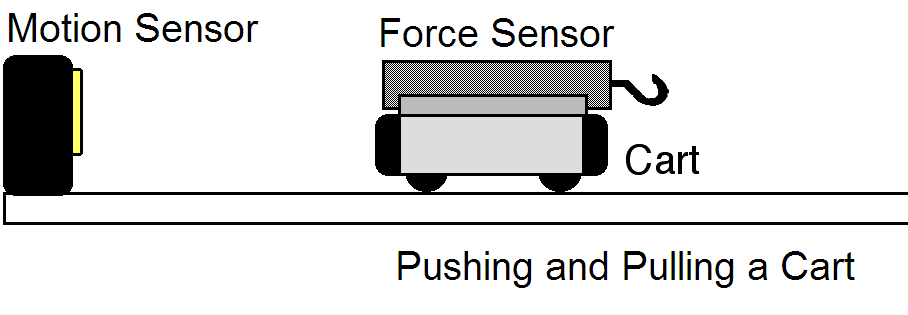
\includegraphics[width=\textwidth]{Force_3_Setup}

\begin{enumerate}
\item
Remove the Photogate Pulley, string, and hanging weights. Leave the dynamics track, cart and Force probe. The Force probe should remain attached to the cart. Add the Motion sensor to the end of the track.
\item
Attach the Motion Sensor to the 850UI.
\item
In ``Hardware Setup" remove the Photogate by clicking on the icon and pressing Delete. Add the Motion Sensor to the appropriate port.
\item
Open a new page by clicking the ``Add Page" button 
\includegraphics{Add_Page}. Double-click ``Graph" from the toolbar on the right.
\item
We will want a Force vs. Acceleration graph for this experiment. For the vertical axis choose ``Force (N)" and for the horizontal axis choose ``Acceleration ($\text{m/s}^2$)."
\end{enumerate}•

\subsection*{Procedure}
\begin{enumerate}
\item
Make sure the track is level. We can check this by  placing a cart on the track. If the cart rolls one way or the other, use the adjustable feet at one end of the track to raise or lower that end until the track is level and the cart does not roll one way or the other.
\item
The minimum distance the Motion Sensor can read is about 15 cm. Make a mark on the track at 20 cm so that we don't get too close to the sensor.
\item
Measure and record the mass of the cart plus the Force Sensor in the data table.
\item
Before recording any data, make sure that Motion Sensor is correctly aligned and has a clear line-of-sight with the cart.
\item
Position the cart an press the tare button on the side of the Force Sensor.
\item
Click Record to begin data collection.
\item
Firmly grasp the hook of the Force Sensor and push and pull the Force Sensor to make the cart move back and forth in a smooth and even motion. Make sure the cart does not get too close to the Motion Sensor.
\item
Click Stop to end the data recording.
\end{enumerate}•

\subsection*{Analysis}
\begin{enumerate}
\item
Rescale the data in the Graph window.
\item
Use a Proportional Fit 
\includegraphics{Curve_Fit} on the data. The constant of proportionality, $A,$ should be the mass $M$ of the cart and Force Sensor together. Record this value in the data table.
\item
\textbf{Print} a copy of this graph for all group members.
\end{enumerate}•

\begin{question}
Why should the constant of proportionality $A$ of the Force vs. Acceleration graph be the object's mass?
\end{question}
\begin{question}
What is the percent discrepancy between the actual and measured mass?
\end{question}

\begin{samepage}
\hrulefill\\ \\
\emph{Chapter~\ref{chap:Force}:} \textbf{Force}
\begin{enumerate}
\item
\textbf{(1)} Title Page
\item
\textbf{(13)} Theory for Setup II only. Include a free body diagram.
\item
\textbf{(6)} Graphs --- One from each setup.
\item
\textbf{(6)} Data Tables --- One from each setup.
\item
\textbf{(6)} Show sample calculations for Setup II.
\item
\textbf{(18)} Answers to all questions.
\end{enumerate}•
\end{samepage}

\newpage
\section{Data Tables}

\subsection*{Setup I}
\begin{doublespace}
\resizebox{1.25\textwidth}{!}{
\begin{tabular}{|c||c|c|c||c|c||c|c|c|}
\hline
Trial & $M$ (kg) & $m$ (kg) & Total Mass (kg) & $a_{th} \text{ (m/s}^2)$ & $a_{exp} \text{ (m/s}^2)$ & $F_{th}$ (N) & $F_{exp}$ (N) & \% Discrepancy\\
\hline
&&&&&&&&\\
\hline
&&&&&&&&\\
\hline
&&&&&&&&\\
\hline
&&&&&&&&\\
\hline
&&&&&&&&\\
\hline
&&&&&&&&\\
\hline
&&&&&&&&\\
\hline
\end{tabular}•
}
\end{doublespace}

\newpage
\subsection*{Setup II}

\begin{doublespace}
\resizebox{0.8\textwidth}{!}{
\begin{tabular}{|l|@{\hskip 2 cm}r|}
\hline
Item & Value\\
\hline
Mass of cart \& sensor $M$ & kg\\
\hline
Mass of hanger \& masses $m$ & kg\\
\hline
Acceleration (slope) $a_{exp}$ & $\text{m/s}^2$\\
\hline
Acceleration (calculated) $a_{th}$ & $\text{m/s}^2$\\
\hline
Force (mean) $T_{exp}$ & N\\
\hline
Force (calculated) $T_1$ & N\\
\hline
Force (calculated) $T_2$ & N\\
\hline
\end{tabular}•
}
\end{doublespace}

\newpage
\subsection*{Setup III}

\begin{doublespace}
\begin{tabular}{|l|@{\hskip 2 cm}r|}
\hline
Item & Value\\
\hline
Mass of cart \& sensor (measured) $M_{th}$ & kg\\
\hline
Mass of cart \& sensor ($A$) $M_{exp}$ & kg\\
\hline
\end{tabular}
\end{doublespace}

\end{document}
